\chapter{PENGUJIAN DAN EVALUASI}
	Pada bab ini akan dibahas uji coba dan evaluasi dari sistem yang telah dibuat. Sistem akan diuji coba fungsionalitas dan performanya dengan menjalankan skenario uji coba yang sudah ditentukan. Uji coba dilakukan untuk mengetahui hasil dari sistem ini sehingga dapat menjawab rumusan masalah pada tugas akhir ini.    
    \section{Lingkungan Uji Coba}
    Uji coba sistem ini dilakukan dengan menggunakan 1 buah komputer sebagai \textit{docker host}, 1 buah komputer sebagai \textit{server} dari halaman \textit{login} sistem, dan 2 komputer sebagai \textit{client}. Semua \textit{client} merupakan virtual komputer menggunakan \textit{VirtualBox}.
    % Please add the following required packages to your document preamble:
% \usepackage{multirow}
% Please add the following required packages to your document preamble:
% \usepackage{multirow}
    \begin{enumerate}
    \item \textbf{Komputer sebagai \textit{Docker Host}}
    \begin{longtable}{|l|l|}
    \caption{Komputer sebagai \textit{Docker Host}}
    \label{DockerHost1} \\
    \hline
    \multirow{3}{*}{\textbf{Perangkat Keras}}      & \begin{tabular}[c]{@{}l@{}} Processor Intel(R) Core(TM) \\ i5-2120 CPU @ 3.30GHz\end{tabular} \\ \cline{2-2} 
    & RAM 8GB	\\ \cline{2-2} 
    & Hard disk 500GB \\ \hline
    \multirow{5}{*}{\textbf{Perangkat Lunak}}      & Linux Mint 18.03 64 bit. \\ \cline{2-2} 
    & Docker versi 1.13.1. \\ \cline{2-2} 
    & MySQL versi 5.7.18. \\ \cline{2-2} 
    & Python versi 3.5.2. \\ \cline{2-2} 
    & Flask versi 1.0.2. \\ \cline{2-2} 
    & VIM versi 7.4.1. \\ \cline{2-2} 
    & Iptables versi 1.6.0. \\ \hline
    \multirow{4}{*}{\textbf{Konfigurasi Jaringan}} & IP address : 10.151.36.38 \\ \cline{2-2} 
    & Netmask : 255.255.255.0 \\ \cline{2-2} 
    & Gateway : 10.151.36.1 \\ \cline{2-2} 
    & Hostname : X450LD \\ \hline
    \end{longtable}
    
    \item \textbf{Komputer sebagai \textit{Server} dari Halaman \textit{Login}}
    \begin{longtable}{|l|l|}
   	\caption{Komputer sebagai \textit{Server} dari Halaman \textit{Login}}
   	\label{DockerHost2} \\
   	\hline
   	\multirow{3}{*}{\textbf{Perangkat Keras}}      & \begin{tabular}[c]{@{}l@{}} Processor Intel(R) Core(TM) \\ i5-2120 CPU @ 3.30GHz\end{tabular} \\ \cline{2-2} 
   	& RAM 1GB	\\ \cline{2-2} 
   	& Hard disk 20GB \\ \hline
   	\multirow{5}{*}{\textbf{Perangkat Lunak}}      & Ubuntu 16.04 64 bit. \\ \cline{2-2} 
   	& Python versi 3.5.2. \\ \cline{2-2} 
   	& Flask versi 1.0.2. \\ \cline{2-2} 
   	& VIM versi 7.4.1. \\ \hline 
   	\multirow{4}{*}{\textbf{Konfigurasi Jaringan}} & IP address : 10.151.36.130 \\ \cline{2-2} 
   	& Netmask : 255.255.255.0 \\ \cline{2-2} 
   	& Gateway : 10.151.36.38 \\ \cline{2-2} 
   	& Hostname : SERVERLOGIN \\ \hline
    \end{longtable}
    
    

    \item \textbf{Komputer sebagai \textit{Client}}
   	\begin{enumerate}

	\item \textbf{\textit{Client} 1}
    \begin{longtable}{|l|l|}
    \caption{\textit{Client} 1}
    \label{DockerHost1} \\
    \hline
    \multirow{3}{*}{\textbf{Perangkat Keras}}      & \begin{tabular}[c]{@{}l@{}} Processor Intel(R) Core(TM) \\ i5-2120 CPU @ 3.30GHz\end{tabular} \\ \cline{2-2} 
    & RAM 1GB	\\ \cline{2-2} 
    & Hard disk 20GB \\ \hline
    \multirow{2}{*}{\textbf{Perangkat Lunak}}      & Linux Ubuntu 16.04 64 bit \\ \cline{2-2} 
    & Firefox Quantum versi 58.0.2. \\ \hline
    \multirow{4}{*}{\textbf{Konfigurasi Jaringan}} & IP address : 192.168.99.100 \\ \cline{2-2} 
    & Netmask : 255.255.255.0 \\ \cline{2-2} 
    & Gateway : 192.168.99.1 \\ \cline{2-2} 
    & Hostname : CLIENT1 \\ \hline
    \end{longtable} 

    \item \textbf{\textit{Client} 2}
    \begin{longtable}{|l|l|}
   	\caption{\textit{Client} 2}
   	\label{DockerHost1} \\
   	\hline
   	\multirow{3}{*}{\textbf{Perangkat Keras}}      & \begin{tabular}[c]{@{}l@{}} Processor Intel(R) Core(TM) \\ i5-2120 CPU @ 3.30GHz\end{tabular} \\ \cline{2-2} 
   	& RAM 1GB	\\ \cline{2-2} 
   	& Hard disk 20GB \\ \hline
   	\multirow{2}{*}{\textbf{Perangkat Lunak}}      & Linux Ubuntu 16.04 64 bit \\ \cline{2-2} 
   	& Firefox Quantum versi 58.0.2. \\ \hline
   	\multirow{4}{*}{\textbf{Konfigurasi Jaringan}} & IP address : 192.168.99.101 \\ \cline{2-2} 
   	& Netmask : 255.255.255.0 \\ \cline{2-2} 
   	& Gateway : 192.168.99.1 \\ \cline{2-2} 
   	& Hostname : CLIENT1 \\ \hline
    \end{longtable}   
    \end{enumerate}
    \end{enumerate}
    
    \section{Skenario Uji Coba}
    Uji Coba ini dilakukan untuk menguji apakah fungsionalitas yang diidentifikasikan pada tahap kebutuhan benar-benar telah diimplementasikan dan bekerja seperti yang seharusnya. Uji coba akan didasarkan pada beberapa skenario untuk menguji kesesuaian respon sistem. Skenario pengujian dibedakan menjadi 2 bagian yaitu:
    \begin{itemize}
    	\item \textbf{Uji Fungsionalitas}
        Pengujian ini didasarkan pada kebutuhan sistem yang telah didasarkan pada kebutuhan sistem yang diidentifikasikan pada bab 3.
        \item \textbf{Uji Performa}
        Pengujian ini digunakan untuk mengukur efisiensi sistem dan performa sistem dalam menjalankankan fungsionalitas sistem.
    \end{itemize}
      \subsection{Skenario Uji Fungsionalitas}
      Uji coba fungsionalitas dilakukan dengan cara menjalankan sistem yang telah dibuat, dan melakukan pengujian terhadap fitur yang telah dibuat. Uji coba fungsionalitas akan berfungsi untuk memastikan sistem sudah memenuhi kebutuhan yang tertera pada Bab 3, yaitu meliputi:
   \begin{enumerate}
      \item Pengujian \textit{client} dapat \textit{login}. ke dalam sistem.
      \item Pengujian \textit{client} dapat mengirimkan permintaan penyediaan kontainer \textit{docker} ke \textit{docker host}.
      \item Pengujian \textit{docker host} dapat menerima perintah penyediaan kontainer \textit{docker}.
      \end{enumerate}
      
\subsubsection{Uji Coba \textit{Client} dapat \textit{Login} ke Dalam Sistem}
Uji coba ini dilakukan oleh \textit{client} dalam keadaan belum \textit{login} ke dalam sistem. Saat \textit{client} mencoba membuka sebuah web http, maka akan langsung diarahkan ke halaman \textit{login} dari sebuah sistem. Saat \textit{client} sudah diarahkan ke halaman \textit{login} sistem, maka \textit{client} harus memasukkan \textit{username} atau NRP mahasiswa dan \textit{password}. Lalu \textit{client} akan mengirim \textit{http requests} kepada \textit{docker host}. Daftar uji fungsionalitas \textit{client} dapat \textit{login} ke dalam sistem dijelaskan pada Tabel \ref{ujicoba1}.

\begin{longtable}{|p{0.03\textwidth}|p{0.25\textwidth}|p{0.21\textwidth}|p{0.35\textwidth}|} % L = Rata kiri untuk setiap kolom, | = garis batas vertikal.
	
% Kepala tabel, berulang di setiap halaman
\caption{Skenario Uji Coba User dapat \textit{Login} ke Dalam Sistem} \label{ujicoba1} \\
\hline
\textbf{No} & \textbf{Routes} & \textbf{Uji Coba} & \textbf{Hasil Harapan} \\ \hline
\endfirsthead
\caption[]{Uji Coba mengirim permintaan penyediaan kontainer}  \\
\hline
\textbf{No} & \textbf{Syslog Agen} & \textbf{Uji Coba} & \textbf{Hasil Harapan} \\ \hline
\endhead
\endfoot
\endlastfoot
% Isi Tabel
1 & /login & Mencocokkan hasil \textit{input username} dan \textit{password} dari \textit{client} dengan basis data yang tersedia. & \textit{client} berhasil \textit{login} ke dalam sistem. \\ \hline
\end{longtable}

\subsubsection{Uji Coba \textit{Client} dapat Mengirimkan Permintaan Penyediaan Kontainer \textit{Docker} ke \textit{Docker Host}}
Uji coba ini dilakukan setelah \textit{client} memasukkan \textit{input username} dan \textit{password}, lalu sistem mencocokkannya dan bernilai benar. Setelah itu, \textit{client} akan mengirim \textit{http requests} kepada \textit{docker host}. Daftar uji fungsionalis \textit{client} dapat mengirimkan permintaan penyediaan kontainer \textit{docker} ke \textit{docker host} dijelaskan pada Tabel \ref{ujicoba2}.

\begin{longtable}{|p{0.03\textwidth}|p{0.25\textwidth}|p{0.21\textwidth}|p{0.35\textwidth}|} % L = Rata kiri untuk setiap kolom, | = garis batas vertikal.
	
% Kepala tabel, berulang di setiap h alaman
\caption{Skenario Uji Coba User dapat \textit{Login} ke Dalam Sistem} \label{ujicoba2} \\
\hline
\textbf{No} & \textbf{Routes} & \textbf{Uji Coba} & \textbf{Hasil Harapan} \\ \hline
\endfirsthead
\caption[]{Uji Coba mengirim permintaan penyediaan kontainer}  \\
\hline
\textbf{No} & \textbf{Syslog Agen} & \textbf{Uji Coba} & \textbf{Hasil Harapan} \\ \hline
\endhead
\endfoot
\endlastfoot
% Isi Tabel
1 & /login & Mengirim request menuju \textit{docker host} melalui browser. & \textit{Request} berhasil diterima oleh \textit{docker host}. \\ \hline
\end{longtable}

\subsubsection{Uji Coba \textit{Docker Host} dapat Menerima Perintah Penyediaan Kontainer \textit{Docker}}
Uji coba ini dilakukan dengan mengakses sistem melalui rute /tests/endpoint. \textit{Client} akan mengirim \textit{http requests} kepada \textit{docker host}. Lalu sistem akan mengirimkan perintah penyediaan kontainer \textit{docker}. Pada pengujian ini, \textit{image} yang digunakan untuk dipasangkan pada setiap kontainer \textit{docker} adalah \textit{image mitmproxy}, yaitu \textit{image} untuk melakukan \textit{blocking} web maupun menulis \textit{log} untuk semua aktifitas dari \textit{client}. Daftar uji fungsionalitas \textit{docker host} dapat memerima perintah penyediaan kontainer \textit{docker} dijelaskan pada Tabel \ref{ujicoba3}.

\begin{longtable}{|p{0.03\textwidth}|p{0.25\textwidth}|p{0.21\textwidth}|p{0.35\textwidth}|} % L = Rata kiri untuk setiap kolom, | = garis batas vertikal.
	
% Kepala tabel, berulang di setiap h alaman
\caption{Skenario Uji Coba \textit{Docker Host} dapat Menerima Perintah Penyediaan Kontainer \textit{Docker}} \label{ujicoba3} \\
\hline
\textbf{No} & \textbf{Routes} & \textbf{Uji Coba} & \textbf{Hasil Harapan} \\ \hline
\endfirsthead
\caption[]{Uji Coba mengirim permintaan penyediaan kontainer}  \\
\hline
\textbf{No} & \textbf{Syslog Agen} & \textbf{Uji Coba} & \textbf{Hasil Harapan} \\ \hline
\endhead
\endfoot
\endlastfoot
% Isi Tabel
1 & /tests/endpoint & Menerima \textit{requests} dari \textit{client} yang menuju ke \textit{docker host} melalui browser. & \textit{Docker Host} dapat menerima perintah penyediaan kontainer \textit{docker} dan menyediakan kontainer \textit{docker} yang diinginkan. \\ \hline
\end{longtable}


      \subsection{Skenario Uji Performa}
      Sistem yang dibuat pada TA ini menggunakan algoritma \textit{analytic hierarchy process} sebagai algoritma pengambilan keputusan untuk menentukan \textit{docker host} terbaik untuk menyediakan kontainer \textit{docker} yang diinginkan. AHP dipakai agar penempatan kontainer pada \textit{docker host} dapat dilakukan secara efisien. Hal ini dilakukan dengan membandingkan ketersediaan sumberdaya pada masing-masing \textit{docker host} dengan bobot priritas masing-masing kriteria sumber daya. Pengujian dilakukan dengan membandingkan hasil kerja sistem yang menggunakan AHP dengan sistem yang menggunakan algortima \textit{round robin} untuk menentukan \textit{docker host} yang akan dipilih untuk menyediakan kontainer. Setelah itu akan dilihat bagaimana performa sistem dengan algoritma AHP yang menggunakan multi kriteria dibandingkan dengan performa sistem yang menggunakan algortima \textit{round robin} yang tidak menggunakan multi kriteria untuk menentukan \textit{docker host} yang akan dipilih. Selain itu pengujian juga akan menggunakan \textit{image docker} variasi yaitu image httpd, nginx, moodle, dan mysql. Image yang bervariasi digunakan agar kebutuhan sumber daya masing-masing \textit{docker host} yang dipakai berbeda-beda untuk setiap image \textit{docker} yang akan dipasangkan pada setiap \textit{docker host}. 
      Selain itu, Uji Performa juga akan menilai kemampuan sistem dengan algoritma AHP bersarkan jumlah kontainer yang akan dipasangkan. Performa sistem akan di evaluasi secara bertahap dengan melihat pertumbuhan penggunan sumber daya pada masing-masing \textit{docker host}. Uji coba performa akan menguji efisiensi sistem dalam menempatkan kontainer \textit{docker} yang diinginkan oleh user pada \textit{docker host} yang ada dan ketepatan sistem dalam menempatkan kontainer \textit{docker} yang diinginkan.
      Arsitektur pengujian tertera pada gambar \ref{skenarioSkalabilitas}
\begin{figure}[H]
        \centering
        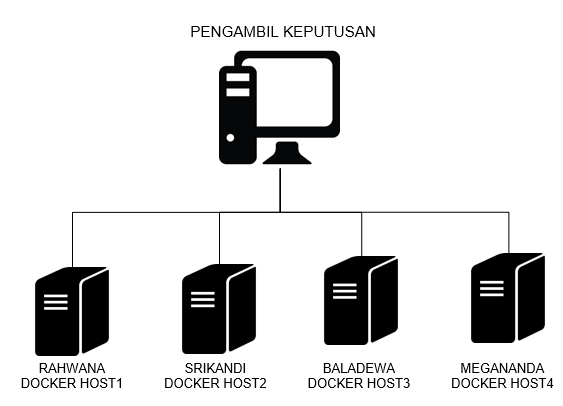
\includegraphics[width=\linewidth]{images/bab5/arsitekturujicoba}
        \caption{Arsitektur Pengujian Performa}
        \label{skenarioSkalabilitas}
      \end{figure} 
    \section{Hasil Uji Coba dan Evaluasi}
    	Berikut dijelaskan hasil uji coba dan evaluasi berdasarkan skenario yang sudah dijelaskan pada bab 5.2.

\subsection{Uji Fungsionalitas}
Berikut dijelaskan hasil pengujian fungsionalitas pada sistem.
\subsubsection{Uji Coba User Mengirim Permintaan Penyediaan Kontainer}
      Uji coba ini dilakukan dengan mengakses sistem melalui rute dan parameter yang telah ditentukan pada Tabel \ref{sUF1}. Pengguna akan mengirim \textit{http request} kepada web service yang telah disediakan pada Komputer Penerima Permintaan Penyediaan Kontainer. Hasil uji coba seperti tertera pada tabel \ref{HsUF1}.
      
      \begin{longtable}{|p{0.03\textwidth}|p{0.25\textwidth}|p{0.21\textwidth}|p{0.35\textwidth}|} % L = Rata kiri untuk setiap kolom, | = garis batas vertikal.

% Kepala tabel, berulang di setiap halaman
\caption{Hasil Skenario Uji Coba mengirim permintaan penyediaan kontainer} \label{HsUF1} \\
\hline
\textbf{No} & \textbf{Routes} & \textbf{Uji Coba} & \textbf{Hasil} \\ \hline
\endfirsthead
\caption[]{Hasil Skenario uji Coba mengirim permintaan penyediaan kontainer}  \\
\hline
\textbf{No} & \textbf{Routes} & \textbf{Uji Coba} & \textbf{Hasil} \\ \hline
\endhead
\endfoot
\endlastfoot
% Isi Tabel
1 & /data/httpd & Mengirim request menuju rute web service melalui browser. & OK. \\ \hline
\end{longtable}	

\subsubsection{Uji Coba Sistem dapat Melakukan Penghitungan AHP}
      Uji coba ini dilakukan dengan mengakses sistem melalui rute yang telah ditentukan pada Tabel \ref{sUF2}. Pengguna akan mengirim \textit{http request} kepada web service yang telah disediakan pada Komputer Penerima Permintaan Penyediaan Kontainer dan sistem akan melakukan penghitungan AHP terhadap data sumber daya setiap \textit{docker host} yang ada sebagai acuan. Hasil uji coba seperti tertera pada Tabel \ref{ujif1.1} dan \ref{ujif1}.
     

\begin{longtable}{|p{0.11\textwidth}|p{0.20\textwidth}|p{0.15\textwidth}|p{0.17\textwidth}|p{0.19\textwidth}|} % L = Rata kiri untuk setiap kolom, | = garis batas vertikal.

% Kepala tabel, berulang di setiap halaman
\caption{Kondisi Awal Penggunaan Sumberdaya \textit{Docker Host} sebelum uji coba dijalankan} \label{ujif1.1} \\
\hline
\textbf{No} & \textbf{Docker Host} & \textbf{CPU} & \textbf{RAM}  & \textbf{Storage} \\ \hline
\endfirsthead
\caption[]{Kondisi Awal Penggunaan Sumberdaya \textit{Docker Host} sebelum uji coba dijalankan}  \\
\hline
\textbf{No} & \textbf{Docker Host} & \textbf{CPU} & \textbf{RAM} & \textbf{Storage} \\ \hline
\endhead
\endfoot
\endlastfoot

% Isi Tabel
1 & RAHWANA & 0.2\%  & 797M/1.9G & 11G/16G \\ \hline
2 & SRIKANDI & 0.3\%  & 532M/2.9G & 8.8G/50G \\ \hline
3 & BALADEWA & 0.1\%  & 354M1.9G/ & 37G/57G \\ \hline
4 & MEGANANDA & 0.1\%  & 555M/1.9G & 10G/16G \\ \hline
\end{longtable}

\begin{longtable}{|p{0.03\textwidth}|p{0.25\textwidth}|p{0.21\textwidth}|p{0.35\textwidth}|} % L = Rata kiri untuk setiap kolom, | = garis batas vertikal.

% Kepala tabel, berulang di setiap halaman
\caption{Hasil Skenario Uji Coba Sistem dapat melakukan Penghitungan AHP} \label{ujif1} \\
\hline
\textbf{No} & \textbf{Docker Host} & \textbf{Uji Coba} & \textbf{Hasil} \\ \hline
\endfirsthead
\caption[]{Hasil Skenario Uji Coba Sistem dapat melakukan Penghitungan AHP}  \\
\hline
\textbf{No} & \textbf{Routes} & \textbf{Uji Coba} & \textbf{Hasil} \\ \hline
\endhead
\endfoot
\endlastfoot
% Isi Tabel
1 & /data/httpd & Mengirim request menuju rute web service melalui browser. & web service berhasil melakukan AHP dan menghasilkan hostname dari \textit{docker host} terpilih, yaitu dalam uji coba ini menghasilkan \textit{hostname} SRIKANDI. \\ \hline
\end{longtable}	

Pada Uji Coba berhasil didapatkan hostname dari \textit{Docker Host} terbaik, yaitu SRIKANDI seperti yang ditunjukkan pada Gambar \ref{gambarujif1}, dikarenakan SRIKANDI memiliki ketersediaan sumber daya yang lebih baik dibanding \textit{Docker Host} lain berdasarkan penghitungan dengan menggunakan algortima AHP.

\begin{figure}[H]
\centering
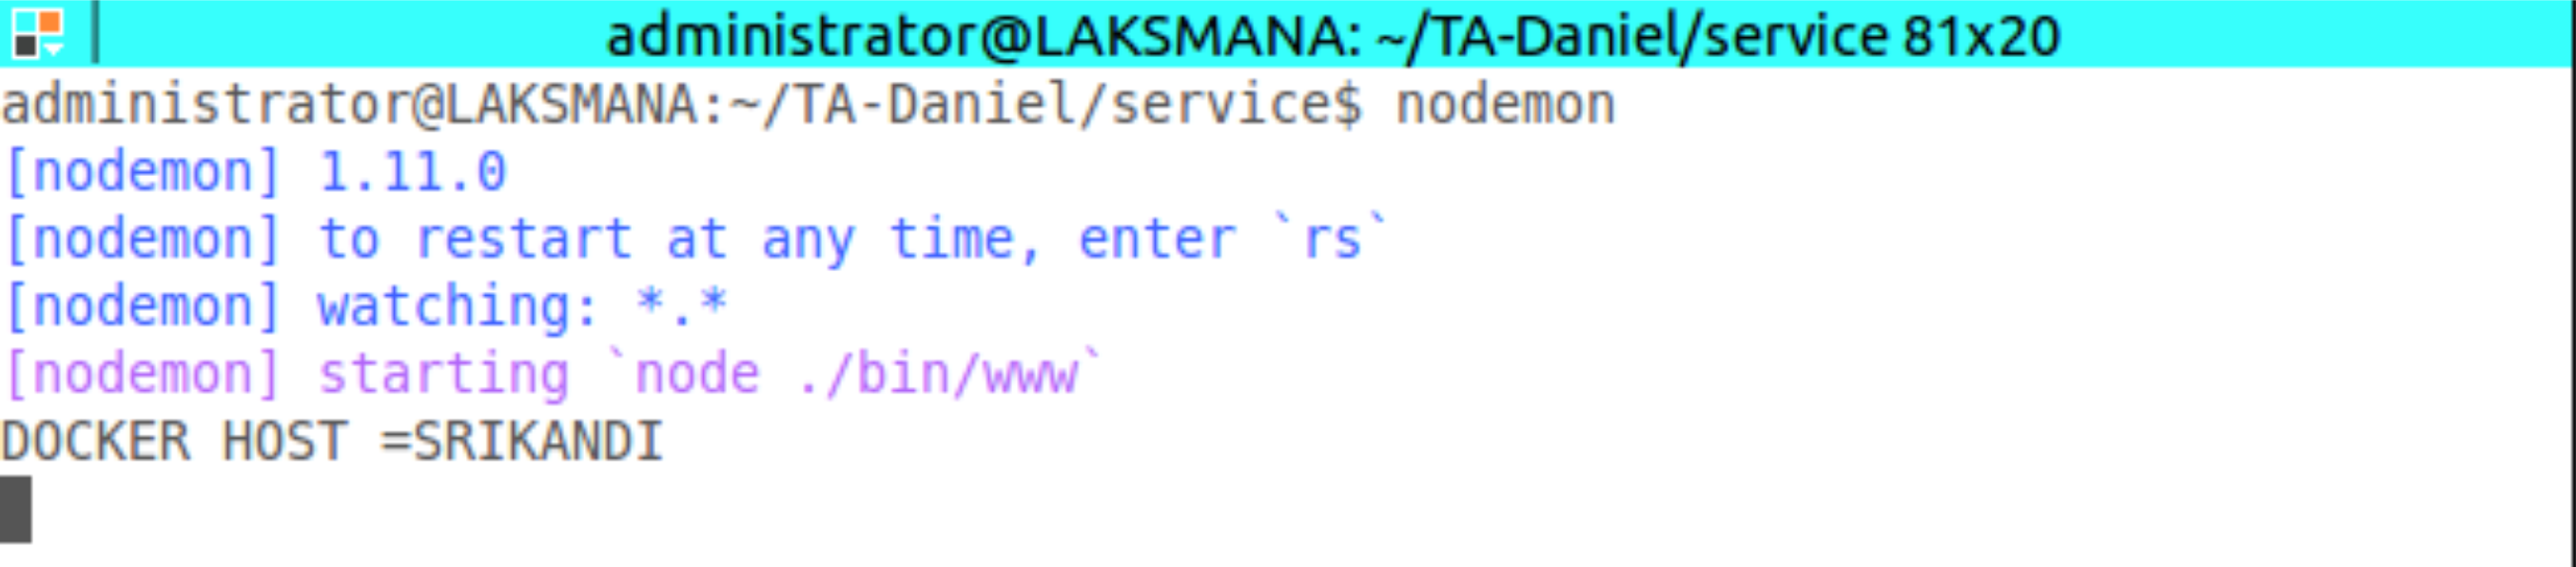
\includegraphics[width=\linewidth]{images/bab5/Selection_005}
\caption{Gambar Hasil Uji Sistem dapat melakukan Penghitungan AHP }
\label{gambarujif1}
\end{figure}     


\subsubsection{Uji Coba \textit{Docker Host} dapat Menerima Perintah Penyediaan Kontainer}
      Uji coba ini dilakukan dengan mengakses sistem melalui rute, parameter  yang telah ditentukan pada Tabel \ref{sUF3}. Pengujian dilakukan image httpd yang akan diujikan pada setiap \textit{docker host}. Hasil uji coba ditunjukkan pada Tabel \ref{Hsuf3}
      
      \begin{longtable}{|p{0.11\textwidth}|p{0.20\textwidth}|p{0.15\textwidth}|p{0.17\textwidth}|p{0.19\textwidth}|} % L = Rata kiri untuk setiap kolom, | = garis batas vertikal.

% Kepala tabel, berulang di setiap halaman
\caption{Hasil Skenario Uji Coba \textit{Docker Host} dapat menerima perintah penyediaan kontainer} \label{Hsuf3} \\
\hline
\textbf{No} & \textbf{Route} & \textbf{Docker Host} & \textbf{Uji Coba} & \textbf{Hasil} \\ \hline
\endfirsthead
\caption[]{Hasil Skenario Uji Coba \textit{Docker Host} dapat menerima perintah penyediaan kontainer}  \\
\hline
\textbf{No} & \textbf{Route} & \textbf{Docker Host} & \textbf{Uji Coba} & \textbf{Hasil} \\ \hline
\endhead
\endfoot
\endlastfoot

% Isi Tabel
1 & /data/httpd & \textit{Docker Host} 1 & Mengirim request penyediaan \textit{docker} dengan image httpd menuju rute web service melalui browser. & \textit{Docker Host} berhasil menerima perintah penyediaan kontainer dan menyediakan kontainer \textit{docker} dengan image httpd. \\ \hline
2 & /data/httpd & \textit{Docker Host} 2 & Mengirim request penyediaan \textit{docker} dengan image httpd menuju rute web service melalui browser. & \textit{Docker Host} berhasil menerima perintah penyediaan kontainer dan menyediakan kontainer \textit{docker} dengan image httpd. \\ \hline
3 & /data/httpd & \textit{Docker Host} 3 & Mengirim request penyediaan \textit{docker} dengan image httpd menuju rute web service melalui browser. & \textit{Docker Host} berhasil menerima perintah penyediaan kontainer dan menyediakan kontainer \textit{docker} dengan image httpd. \\ \hline
4 & /data/httpd & \textit{Docker Host} 4 & Mengirim request penyediaan \textit{docker} dengan image httpd menuju rute web service melalui browser. & \textit{Docker Host} berhasil menerima perintah penyediaan kontainer dan menyediakan kontainer \textit{docker} dengan image httpd. \\ \hline
\end{longtable}
Pada Gambar \ref{perintahansible} dan Gambar \ref{dockerterpasang} ditunjukkan bagaimana kondisi saat sistem menghasilkan perintah untuk menyediakan \textit{docker} dan saat \textit{docker} sudah terpasang pada \textit{docker host}

\begin{figure}[H]
\centering
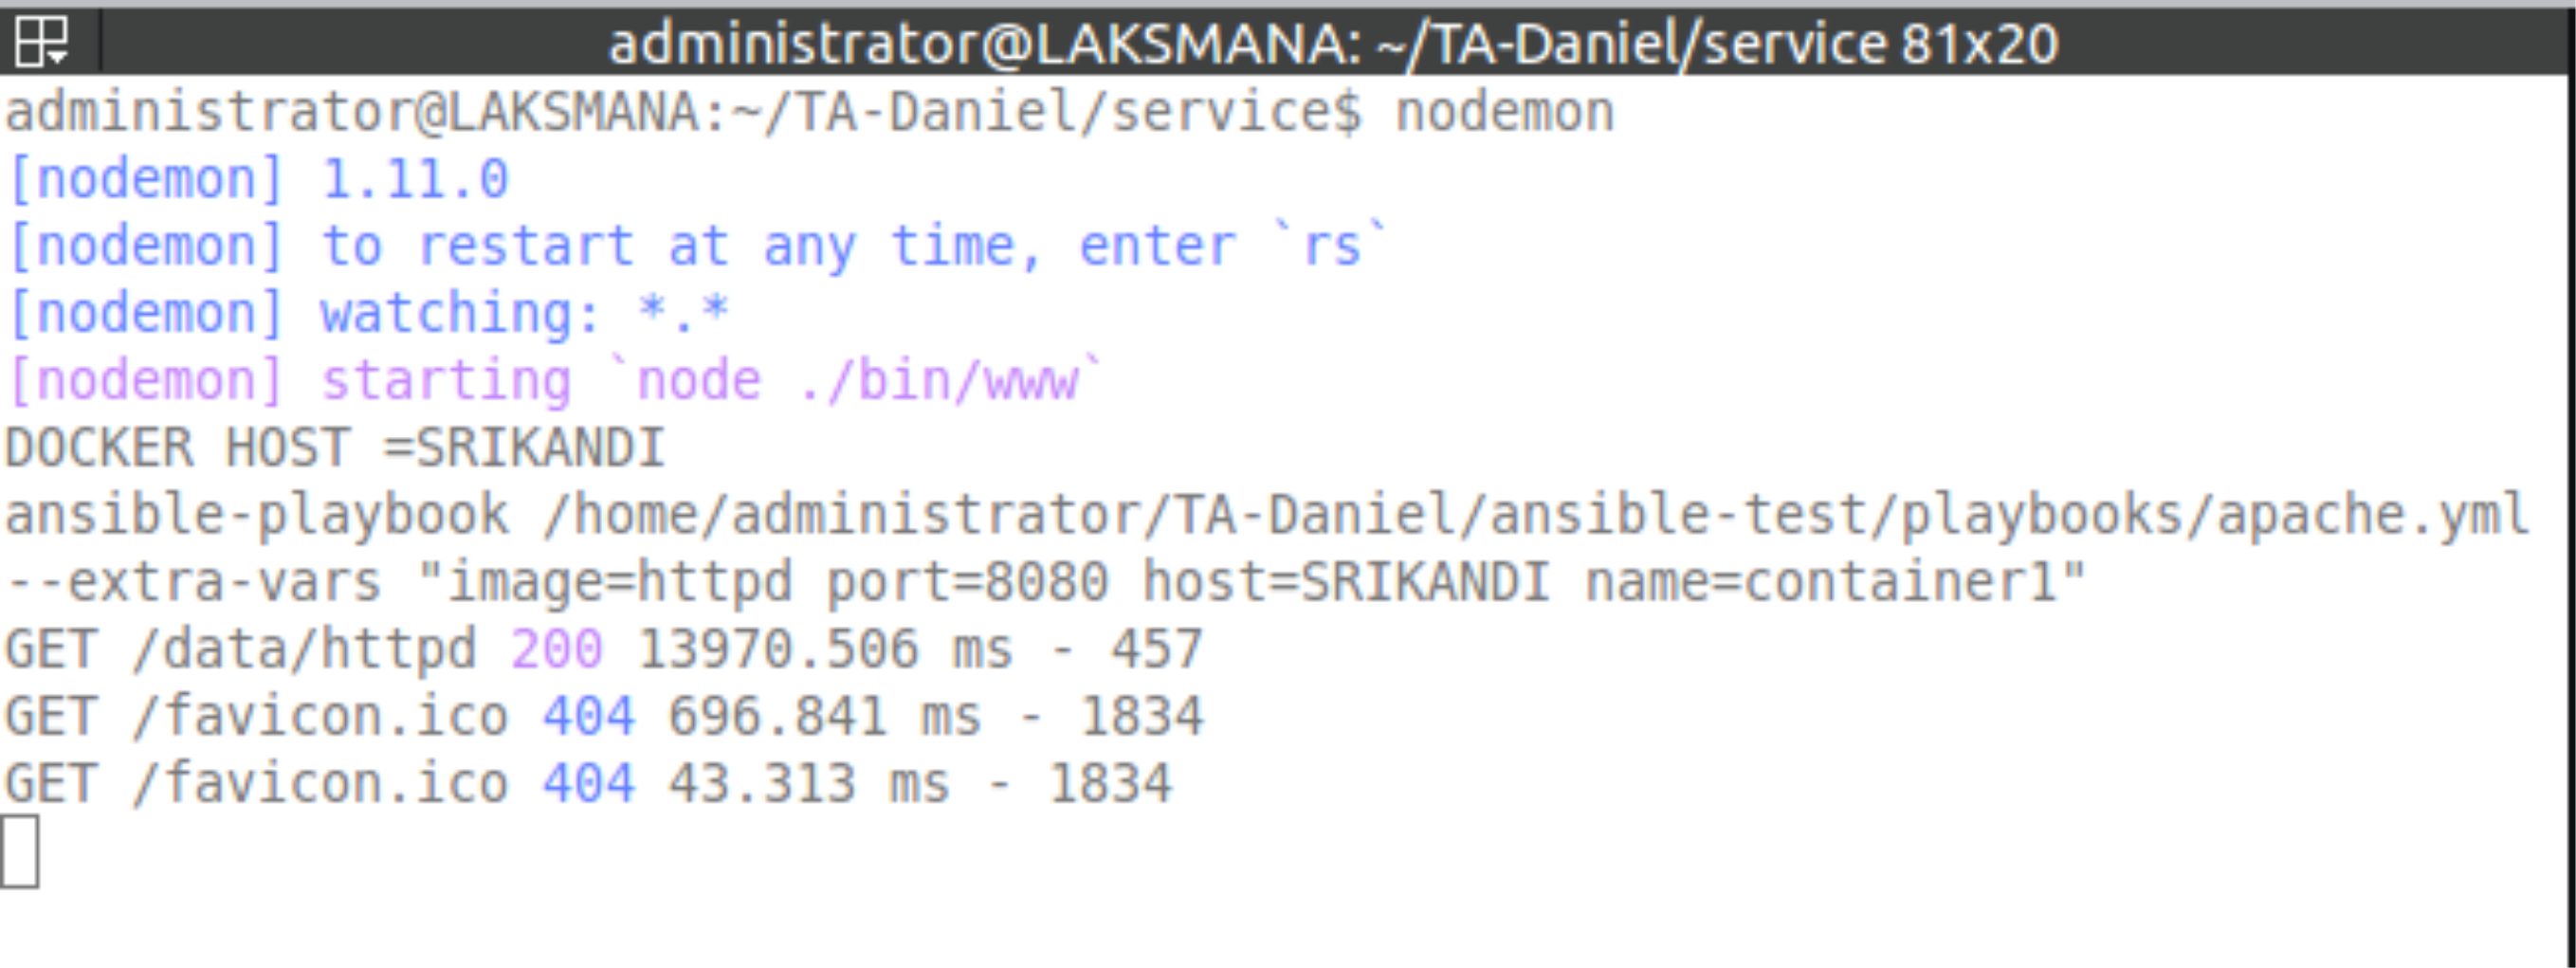
\includegraphics[width=\linewidth]{images/bab5/Selection_006}
\caption{Web Service Mengrimkan perintah penyediaan kontainer}
\label{perintahansible}
\end{figure}     

\begin{figure}[H]
\centering
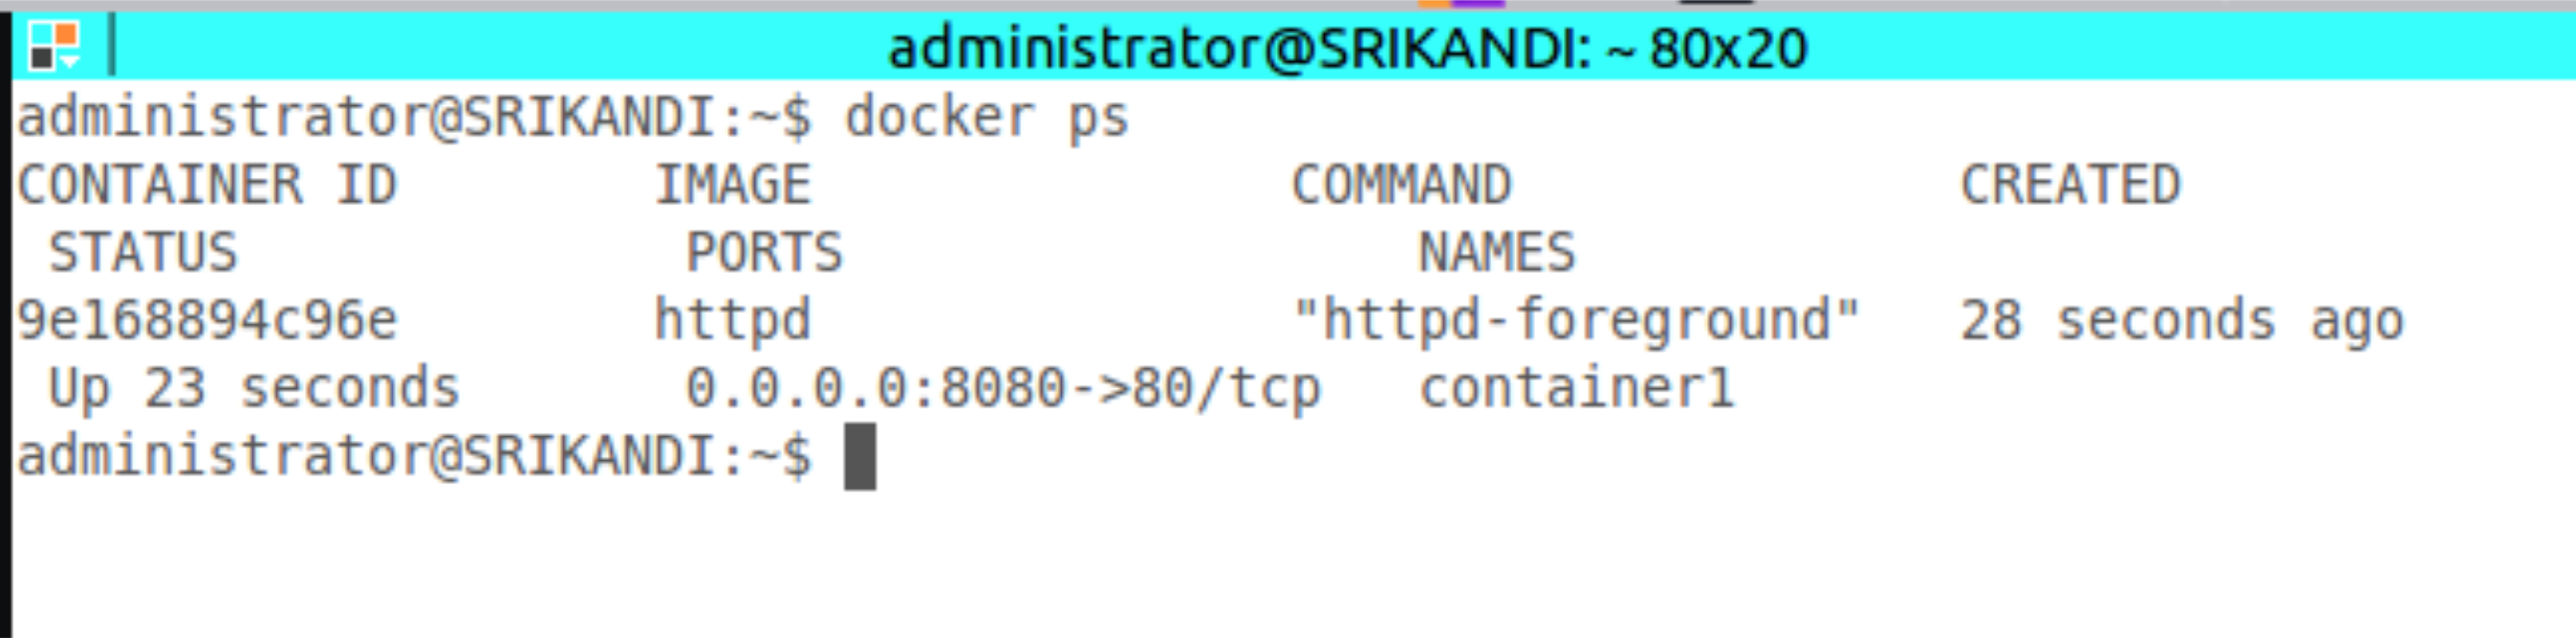
\includegraphics[width=\linewidth]{images/bab5/Selection_007}
\caption{\emph{Docker Host} berhasil membuat kontainer \emph{docker}}
\label{dockerterpasang}
\end{figure}     

\subsubsection{Uji Coba \textit{Docker Host} dapat Mengirim Data Resourcenya Masing-Masing}
      Dilakukan pengujian pada setiap \textit{docker host}. Setiap \textit{docker host} akan mengirimkan data ketersediaan sumber daya CPU, RAM dan File Storage nya masing-masing ke InfluxDB yang terdapat pada \textit{middleware}. Hasil ditunjukkan pada Tabel \ref{HsUF4} 
      
      \begin{longtable}{|p{0.03\textwidth}|p{0.25\textwidth}|p{0.21\textwidth}|p{0.35\textwidth}|} % L = Rata kiri untuk setiap kolom, | = garis batas vertikal.

% Kepala tabel, berulang di setiap halaman
\caption{Hasil Skenario Uji Coba \textit{Docker Host} dapat Mengirim Data Resourcenya Masing-Masing} \label{HsUF4} \\
\hline
\textbf{No} & \textbf{Docker Host} & \textbf{Uji Coba} & \textbf{Hasil } \\ \hline
\endfirsthead
\caption[]{Hasil Skenario uji Coba \textit{Docker Host} dapat Mengirim Data Resource}  \\
\hline
\textbf{No} & \textbf{Docker Host} & \textbf{Uji Coba} & \textbf{Hasil } \\ \hline
\endhead
\endfoot
\endlastfoot
% Isi Tabel
1 & \textit{Docker Host} 1 & Mengirim data sumber daya (RAM, CPU dan \textit{File Storage}) ke InfluxDB pada \textit{middleware} . & Data sumber daya CPU, RAM dan File Storage berhasilkan dikirimkan dan tersimpan pada InfluxDB. \\ \hline
2 & \textit{Docker Host} 2 & Mengirim data sumber daya (RAM, CPU dan \textit{File Storage}) ke InfluxDB pada \textit{middleware} . & Data sumber daya CPU, RAM dan File Storage berhasilkan dikirimkan dan tersimpan pada InfluxDB. \\ \hline
3 & \textit{Docker Host} 3 & Mengirim data sumber daya (RAM, CPU dan \textit{File Storage}) ke InfluxDB pada \textit{middleware} . & Data sumber daya CPU, RAM dan File Storage berhasilkan dikirimkan dan tersimpan pada InfluxDB. \\ \hline
4 & \textit{Docker Host} 4 & Mengirim data sumber daya (RAM, CPU dan \textit{File Storage}) ke InfluxDB pada \textit{middleware} . & Data sumber daya CPU, RAM dan File Storage berhasilkan dikirimkan dan tersimpan pada InfluxDB. \\ \hline
\end{longtable}	      
Sesuai dengan Gambar \ref{DataCpu},\ref{DataRam} dan \ref{DataDf}, ,semua \textit{docker host} berhasil mengirimkan data sumber daya CPU, RAM dan File Storage nya masing-masing ke InfluxDB.
\begin{itemize}
\item Data CPU Setiap Docker Host pada InfluxDB
\begin{figure}[H]
        \centering
        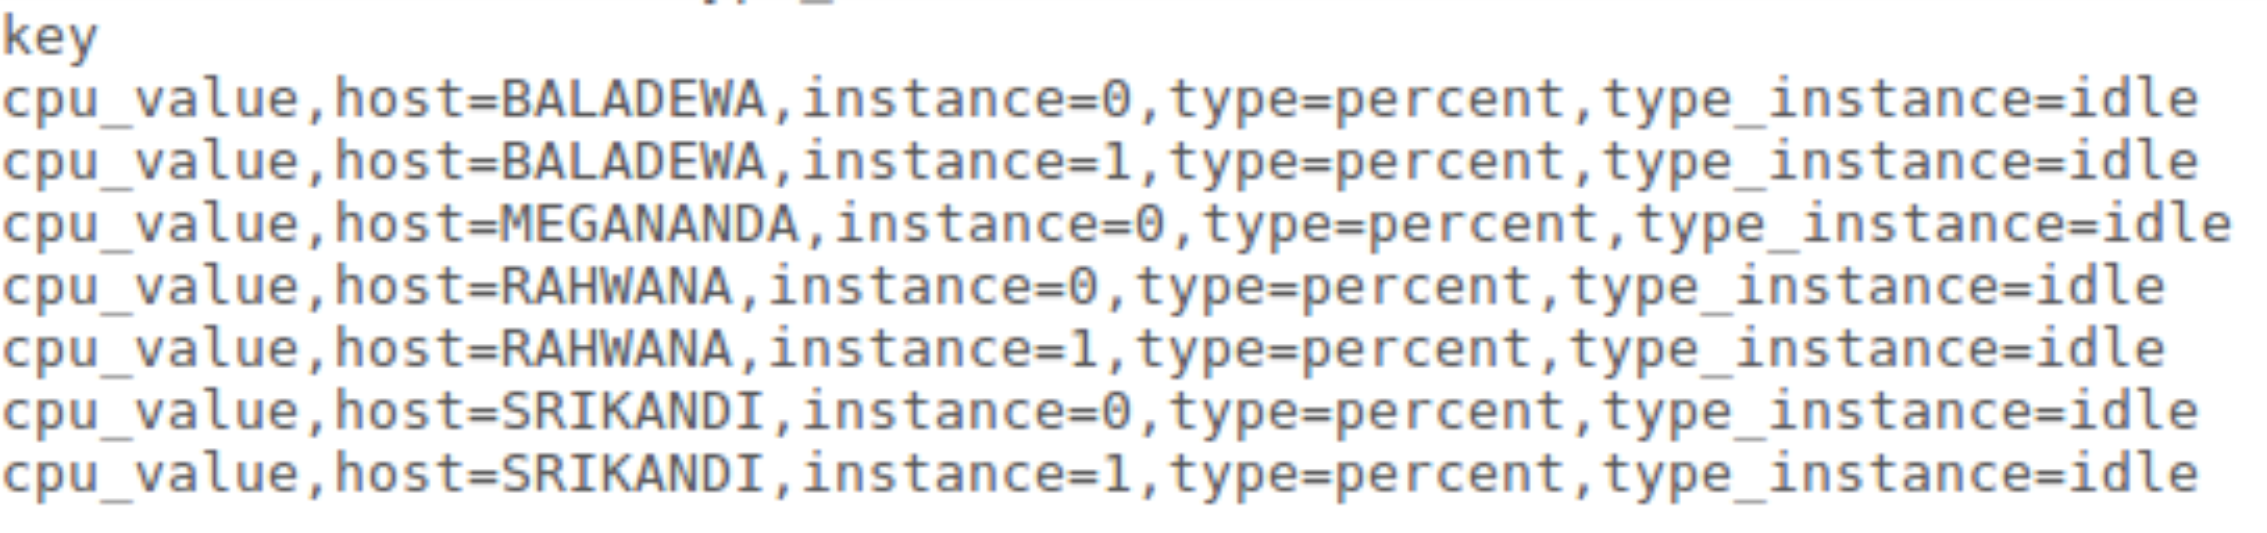
\includegraphics[width=\linewidth]{images/bab5/datacpu}
        \caption{Data CPU Setiap Docker Host pada InfluxDB}
        \label{DataCpu}
      \end{figure} 
\end{itemize}
\begin{itemize}
\item Data RAM Setiap Docker Host pada InfluxDB
\begin{figure}[H]
        \centering
        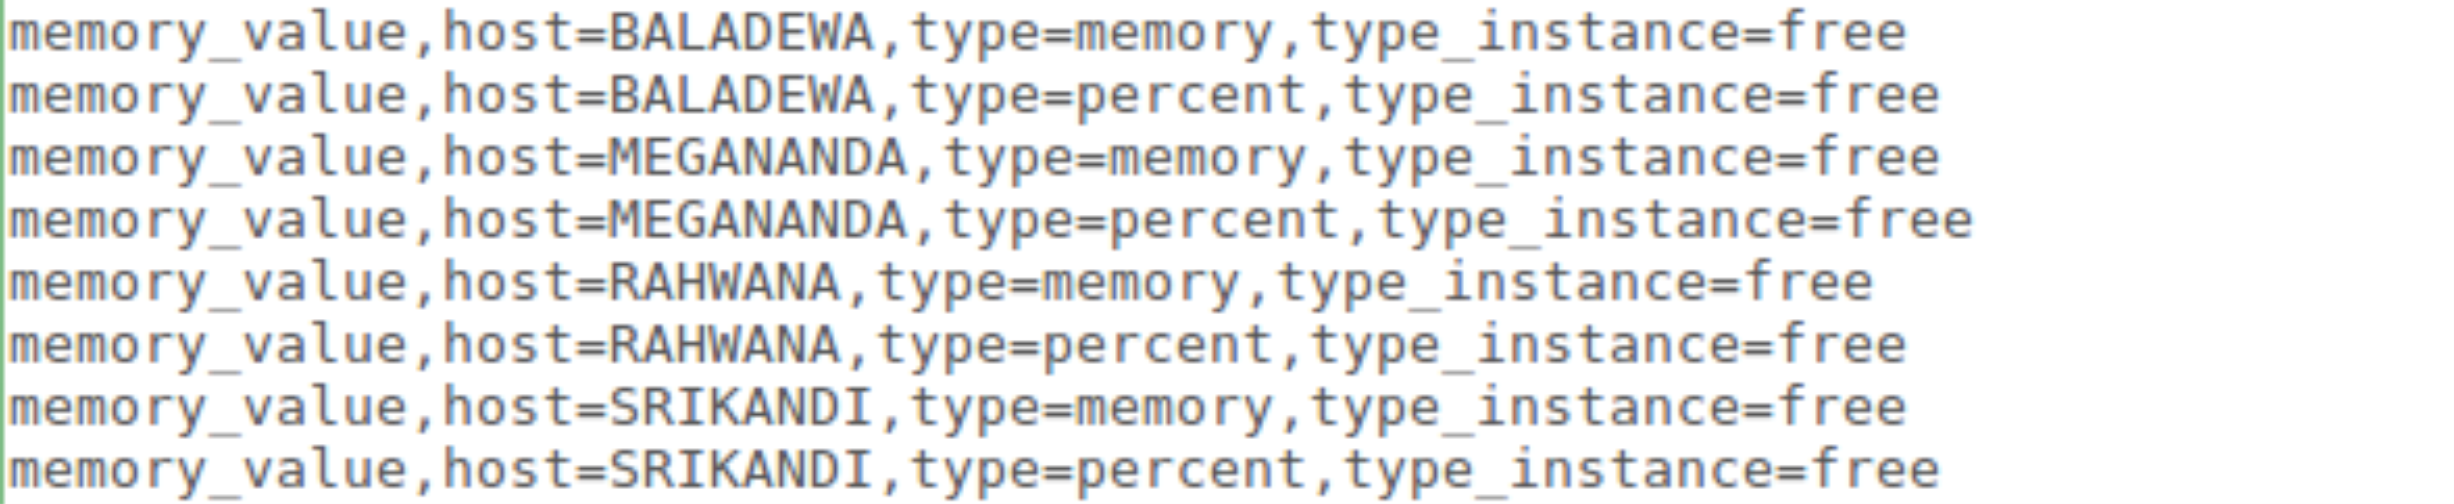
\includegraphics[width=\linewidth]{images/bab5/dataram}
        \caption{Data RAM Setiap Docker Host pada InfluxDB}
        \label{DataRam}
      \end{figure} 
\end{itemize}
\begin{itemize}
\item Data Penyimpanan File Setiap Docker Host pada InfluxDB
\begin{figure}[H]
        \centering
        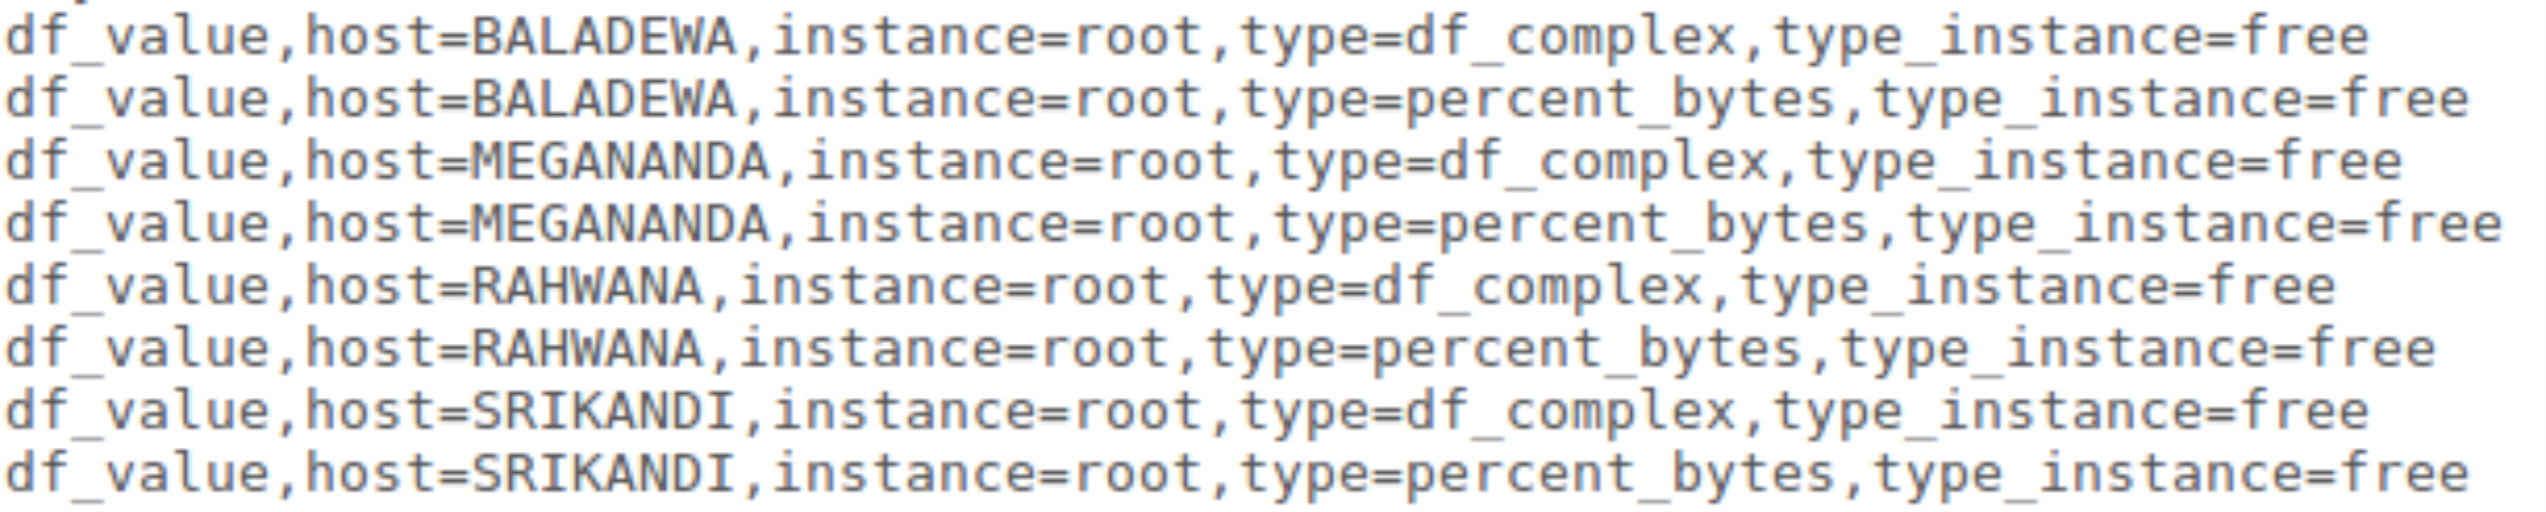
\includegraphics[width=\linewidth]{images/bab5/datadf}
        \caption{Data Penyimpanan File Setiap Docker Host pada InfluxDB}
        \label{DataDf}
      \end{figure} 
\end{itemize}


      \subsection{Uji Performa}
 Seperti yang dijelaskan pada bab 5.2 pengujian performa akan dilakukan pada 4 \textit{docker host} yang tersedia dengan menggunakan sistem yang ada, namun dengan 2 algoritma yang berbeda yaitu menggunakan algoritma pengambilan keputusan AHP dan menggunakan algoritma pembagian kerja dasar, \textit{round robin}\cite{shreedhar_efficient_1996}. Selain itu pengujian juga akan menggunakan beberapa image \textit{docker} yang akan di pasangkan pada setiap \textit{docker host} yang tersedia. Pengujian akan dijalankan dengan mengirimkan permintaan penyediaan kontainer pada sistem dengan jumlah permintaan penyediaan kontainer yang beragam.

\subsubsection{Pengujian Dengan Algoritma AHP}
Kondisi awal ketersediaan sumberdaya \textit{docker host} sebelum uji coba sistem dengan image \textit{docker} httpd dan nginx menggunakan AHP dijalankan ditunjukkan pada Tabel \ref{kondisiawal1}.
\begin{longtable}{|p{0.08\textwidth}|p{0.24\textwidth}|p{0.15\textwidth}|p{0.17\textwidth}|p{0.19\textwidth}|} % L = Rata kiri untuk setiap kolom, | = garis batas vertikal.

% Kepala tabel, berulang di setiap halaman
\caption{Kondisi Awal Ketersediaan Sumberdaya \textit{Docker Host} sebelum uji coba dijalankan} \label{kondisiawal1} \\
\hline
\textbf{No} & \textbf{Docker Host} & \textbf{CPU} & \textbf{RAM}  & \textbf{Storage} \\ \hline
\endfirsthead
\caption[]{Kondisi Awal Ketersediaan Sumberdaya \textit{Docker Host} Sebelum Uji Coba Dijalankan}  \\
\hline
\textbf{No} & \textbf{Docker Host} & \textbf{CPU} & \textbf{RAM} & \textbf{Storage} \\ \hline
\endhead
\endfoot
\endlastfoot

% Isi Tabel
1 & RAHWANA & 98\%  & 1.3G/1.9G & 5G/16G \\ \hline
2 & SRIKANDI & 93\%  & 2.3G/2.9G & 41.2G/50G \\ \hline
3 & BALADEWA & 99\%  & 1G/1.9G & 20G/57G \\ \hline
4 & MEGANANDA & 91\%  & 1.3G/1.9G & 6G/16G \\ \hline
\end{longtable}

Hasil pengujian sistem dengan algoritma AHP menggunakan \textit{image docker} httpd dan nginx ditunjukkan pada Tabel \ref{Uji Performa1}.
\begin{longtable}{|p{0.05\textwidth}|p{0.15\textwidth}|p{0.15\textwidth}|p{0.15\textwidth}|p{0.15\textwidth}|p{0.15\textwidth}|}
\caption{Hasil Uji Coba Performa sistem dengan \textit{Image Docker} httpd dan nginx menggunakan AHP}
\label{Uji Performa1} \\
\hline
\multirow{2}{*}{No} & \multirow{2}{*}{\begin{tabular}[c]{@{}c@{}}Jumlah\\ Kontainer\end{tabular}} & \multicolumn{4}{c|}{Kontainer Terpasang pada \textit{Docker Host}} \\ \cline{3-6} 
  & 	& Rahwana  & Srikandi  & Baladewa & Megananda    \\ \hline
1 & 254 & 39       & 135       & 27       & 53       \\ \hline
2 & 254 & 40       & 131       & 32       & 51       \\ \hline
3 & 254 & 37       & 147       & 20       & 50       \\ \hline
4 & 254 & 41       & 143       & 23       & 47       \\ \hline
5 & 254 & 49       & 132       & 24       & 49       \\ \hline
\end{longtable}  

Kondisi akhir  ketersediaan sumber daya \textit{docker host} pada pengujian sistem dengan algoritma AHP menggunakan \textit{image docker} httpd dan nginx ditunjukkan pada Tabel \ref{kondisiakhir1}.
\begin{longtable}{|p{0.08\textwidth}|p{0.24\textwidth}|p{0.15\textwidth}|p{0.17\textwidth}|p{0.19\textwidth}|} % L = Rata kiri untuk setiap kolom, | = garis batas vertikal.

% Kepala tabel, berulang di setiap halaman
\caption{Rata-rata Kondisi Akhir Ketersediaan Sumberdaya \textit{Docker Host} Setelah Uji Coba Dijalankan} \label{kondisiakhir1} \\
\hline
\textbf{No} & \textbf{Docker Host} & \textbf{CPU} & \textbf{RAM}  & \textbf{Storage} \\ \hline
\endfirsthead
\caption[]{Rata-rata Kondisi Akhir Ketersediaan Sumberdaya \textit{Docker Host} Setelah Uji Coba Dijalankan}  \\
\hline
\textbf{No} & \textbf{Docker Host} & \textbf{CPU} & \textbf{RAM} & \textbf{Storage} \\ \hline
\endhead
\endfoot
\endlastfoot

% Isi Tabel
1 & RAHWANA & 90\%  & 628M/1.9G & 5G/16G \\ \hline
2 & SRIKANDI & 85\%  & 708M/2.9G & 41.2G/50G \\ \hline
3 & BALADEWA & 92\%  & 832M/1.9G & 20G/57G \\ \hline
4 & MEGANANDA & 90\%  & 654M/1.9G & 6G/16G \\ \hline
\end{longtable}

\subsubsection{Pengujian Dengan Algoritma \textit{Round Robin}}
Kondisi awal ketersediaan sumberdaya \textit{docker host} sebelum uji coba sistem dengan \textit{image docker} httpd dan nginx menggunakan \textit{round robin} dijalankan ditunjukkan pada Tabel \ref{kondisiawal2}.
\begin{longtable}{|p{0.08\textwidth}|p{0.24\textwidth}|p{0.15\textwidth}|p{0.17\textwidth}|p{0.19\textwidth}|} % L = Rata kiri untuk setiap kolom, | = garis batas vertikal.

% Kepala tabel, berulang di setiap halaman
\caption{Kondisi Awal Ketersediaan Sumberdaya \textit{Docker Host} Sebelum Uji Coba Dijalankan} \label{kondisiawal2} \\
\hline
\textbf{No} & \textbf{Docker Host} & \textbf{CPU} & \textbf{RAM}  & \textbf{Storage} \\ \hline
\endfirsthead
\caption[]{Kondisi Awal Ketersediaan Sumberdaya \textit{Docker Host} Sebelum Uji Coba Dijalankan}  \\
\hline
\textbf{No} & \textbf{Docker Host} & \textbf{CPU} & \textbf{RAM} & \textbf{Storage} \\ \hline
\endhead
\endfoot
\endlastfoot

% Isi Tabel
1 & RAHWANA & 98\%  & 1.2G/1.9G & 5G/16G \\ \hline
2 & SRIKANDI & 93\%  & 2.3G/2.9G & 41.2G/50G \\ \hline
3 & BALADEWA & 99\%  & 1G/1.9G & 20G/57G \\ \hline
4 & MEGANANDA & 91\%  & 1.4G/1.9G & 6G/16G \\ \hline
\end{longtable}

Hasil dari pengujian sistem dengan algoritma \textit{round robin} ditunjukkan pada Tabel \ref{Uji Performa2}.
\begin{longtable}{|p{0.05\textwidth}|p{0.15\textwidth}|p{0.15\textwidth}|p{0.15
\textwidth}|p{0.15\textwidth}|p{0.15\textwidth}|}
\caption{Hasil Uji Coba Performa Sistem dengan \textit{Image Docker} httpd dan nginx Menggunakan \textit{Round Robin}}
\label{Uji Performa2} \\
\hline
\multirow{2}{*}{No} & \multirow{2}{*}{\begin{tabular}[c]{@{}c@{}}Jumlah\\ Kontainer\end{tabular}} & \multicolumn{4}{c|}{Kontainer Terpasang pada Docker Host} \\ \cline{3-6} 
  &		& Rahwana  & Srikandi & Baladewa & Megananda    \\ \hline
1 & 254 & 63       & 63       & 63       & 63       \\ \hline
2 & 254 & 63       & 63       & 63       & 63       \\ \hline
3 & 254 & 63       & 63       & 63       & 63       \\ \hline
4 & 254 & 63       & 63       & 63       & 63       \\ \hline
5 & 254 & 63       & 63       & 63       & 63       \\ \hline
\end{longtable}
Kondisi akhir ketersediaan sumberdaya \textit{docker host} pada pengujian sistem dengan algoritma \textit{round robin} menggunakan \textit{image docker} httpd dan nginx ditunjukkan pada Tabel \ref{kondisiakhir2}.
\begin{longtable}{|p{0.08\textwidth}|p{0.22\textwidth}|p{0.15\textwidth}|p{0.17\textwidth}|p{0.19\textwidth}|} % L = Rata kiri untuk setiap kolom, | = garis batas vertikal.

% Kepala tabel, berulang di setiap halaman
\caption{Kondisi Akhir Ketersediaan Sumberdaya \textit{Docker Host} Setelah Uji Coba Dijalankan} \label{kondisiakhir2} \\
\hline
\textbf{No} & \textbf{Docker Host} & \textbf{CPU} & \textbf{RAM}  & \textbf{Storage} \\ \hline
\endfirsthead
\caption[]{Kondisi Akhir Ketersediaan Sumberdaya \textit{Docker Host} Setelah Uji Coba Dijalankan}  \\
\hline
\textbf{No} & \textbf{Docker Host} & \textbf{CPU} & \textbf{RAM} & \textbf{Storage} \\ \hline
\endhead
\endfoot
\endlastfoot

% Isi Tabel
1 & RAHWANA & 92\%  & 161M/1.9G & 5G/16G \\ \hline
2 & SRIKANDI & 93\%  & 1.3G/2.9G & 41.1G/50G \\ \hline
3 & BALADEWA & 92\%  & 95M/1.9G & 20G/57G \\ \hline
4 & MEGANANDA & 91\%  & 335M/1.9G & 6G/16G \\ \hline
\end{longtable}  

\subsubsection{Pengujian Performa Sistem dengan Algoritma AHP Berdasarkan Jumlah Kontainer yang Akan Dipasangkan}
Kondisi awal ketersediaan sumberdaya \textit{docker host} sebelum uji coba ditunjukkan pada Tabel \ref{kondisiawal3}.
\begin{longtable}{|p{0.08\textwidth}|p{0.24\textwidth}|p{0.15\textwidth}|p{0.17\textwidth}|p{0.19\textwidth}|} % L = Rata kiri untuk setiap kolom, | = garis batas vertikal.

% Kepala tabel, berulang di setiap halaman
\caption{Kondisi Awal Ketersediaan Sumberdaya \textit{Docker Host} Sebelum Uji Coba Dijalankan} \label{kondisiawal3} \\
\hline
\textbf{No} & \textbf{Docker Host} & \textbf{CPU} & \textbf{RAM}  & \textbf{Storage} \\ \hline
\endfirsthead
\caption[]{Kondisi Awal Ketersediaan Sumberdaya \textit{Docker Host} Sebelum Uji Coba Dijalankan}  \\
\hline
\textbf{No} & \textbf{Docker Host} & \textbf{CPU} & \textbf{RAM} & \textbf{Storage} \\ \hline
\endhead
\endfoot
\endlastfoot

% Isi Tabel
1 & RAHWANA & 99\%  & 1.3G/1.9G & 3.8G/16G \\ \hline
2 & SRIKANDI & 99\%  & 2.3G/2.9G & 37G/50G \\ \hline
3 & BALADEWA & 99\%  & 1G/1.9G & 16G/57G \\ \hline
4 & MEGANANDA & 99\%  & 1.4G/1.9G & 3.8G/16G \\ \hline
\end{longtable}
Hasil pengujian sistem dengan algoritma AHP menggunakan \textit{docker image} httpd, nginx, moodle, dan mysql ditunjukkan pada Table \ref{Uji Performa3}.
\begin{longtable}{|p{0.05\textwidth}|p{0.15\textwidth}|p{0.15\textwidth}|p{0.15\textwidth}|p{0.15\textwidth}|p{0.15\textwidth}|}
\caption{Hasil Uji Coba Performa Sistem dengan \textit{Docker Image} httpd dan nginx Menggunakan AHP}
\label{Uji Performa3} \\
\hline
\multirow{2}{*}{No} & \multirow{2}{*}{\begin{tabular}[c]{@{}c@{}}Jumlah\\ Kontainer\end{tabular}} & \multicolumn{4}{c|}{Kontainer Terpasang pada Docker Host} \\ \cline{3-6} 
  &	 	& Rahwana   & Srikandi & Baladewa & Megananda    \\ \hline
1 & 30  & 0       	& 30       & 0        & 0       \\ \hline
2 & 60 	& 3       	& 55       & 0        & 2       \\ \hline
3 & 100 & 5       	& 73       & 0        & 12       \\ \hline
4 & 120 & 11       	& 88       & 5        & 16       \\ \hline
5 & 150 & 34       	& 46       & 33       & 37       \\ \hline
\end{longtable} 
Kondisi akhir ketersediaan sumberdaya \textit{docker host} setelah uji coba dijalankan ditunjukkan pada Gambar \ref{Grafik CPU RAHWANA} untuk ketersediaan CPU, Gambar \ref{Grafik RAM RAHWANA} untuk ketersediaan Memori dan Gambar \ref{Grafik DF RAHWANA} untuk ketersediaan penyimpaan berkas. 
\begin{figure}[H]
        \centering
        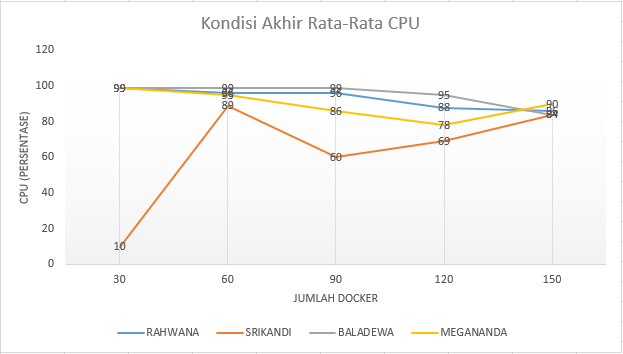
\includegraphics[width=\linewidth]{images/bab5/cpu}
        \caption{Grafik Kondisi Akhir Ketersediaan Rata-Rata CPU}
        \label{Grafik CPU RAHWANA}
      \end{figure} 
\begin{figure}[H]
        \centering
        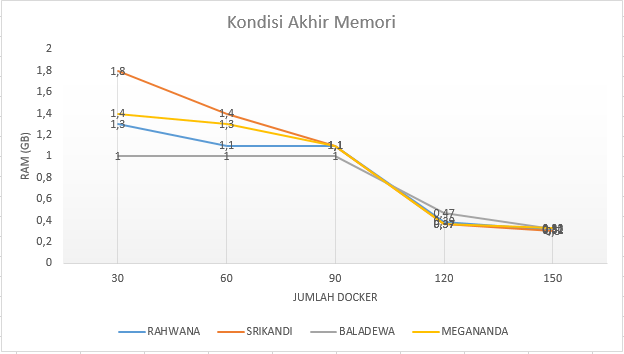
\includegraphics[width=\linewidth]{images/bab5/memori}
        \caption{Grafik Kondisi Akhir Ketersediaan Memori}
        \label{Grafik RAM RAHWANA}
      \end{figure} 
\begin{figure}[H]
        \centering
        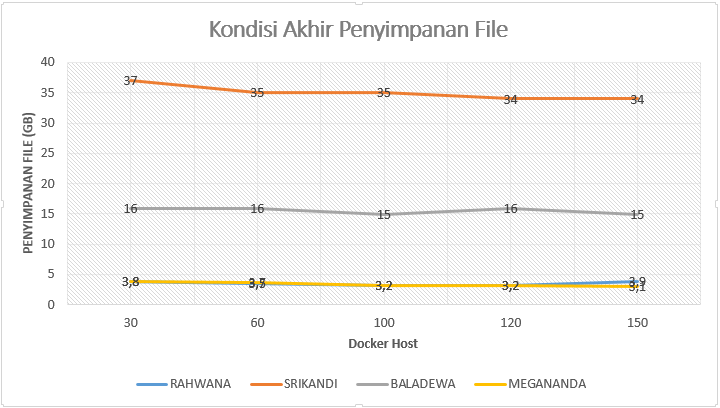
\includegraphics[width=\linewidth]{images/bab5/Storage}
        \caption{Grafik Kondisi Akhir Ketersedian Penyimpaanan FIle}
        \label{Grafik DF RAHWANA}
      \end{figure} 

Waktu Pendistribusian Docker oleh Sistem Berdasarkan Jumlah Kontainer ditunjukkan pada Gambar \ref{Grafik Waktu}
\begin{figure}[H]
        \centering
        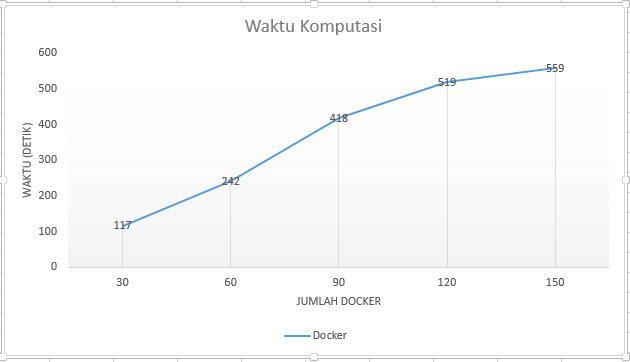
\includegraphics[width=\linewidth]{images/bab5/waktu}
        \caption{Grafik Waktu Pendistribusian Docker oleh Sistem Berdasarkan Jumlah Kontainer}
        \label{Grafik Waktu}
      \end{figure} 

	Dari data hasil uji coba yang didapat, dapat dilihat bahwa algoritma AHP dapat membagikan kontainer ke \textit{docker host} yang ada dengan lebih efisien. Dibandingkan dengan algoritma \textit{round robin} yang menyebarkan kontainer merata ke setiap \textit{docker host}, sistem dengan AHP menghasilkan kondisi ketersediaan sumber daya yang lebih merata pada akhir uji coba. Selain itu pendistribusian pada setiap \textit{docker host} juga memiliki ketepatan yang baik, hal ini terlihat pada saat akan mendistribusikan 30 kontainer, sistem dengan AHP mendistribusikan seluruh kontainer tersebut pada \textit{docker host} SRIKANDI, hal ini disebabkan SRIKANDI memiliki ketersediaan yang jauh lebih dominan dibanding \textit{docker host} yang lain.  Namun, kondisi dimana \textit{docker image} yang bervariasi menimbulkan hasil akhir dari uji coba tidak linear, hal ini disebabkan variasi dari \textit{docker image} akan membuat kebutuhan sumber daya yang dibutuhkan dari setiap \textit{docker host} juga bervariasi.
